\documentclass[12pt, a4paper, titlepage]{article}

\usepackage{qtree} %for trees
\usepackage{amsthm} %for proofs
\usepackage{amsmath}
\usepackage{amsmath}
\usepackage{amssymb}
\usepackage{amsfonts}
\usepackage{amsthm}
\usepackage{tikz}
\usetikzlibrary{automata,positioning}

\newtheoremstyle{break}% name
  {}%         Space above, empty = `usual value'
  {}%         Space below
  {\itshape}% Body font
  {}%         Indent amount (empty = no indent, \parindent = para indent)
  {\bfseries}% Thm head font
  {.}%        Punctuation after thm head
  {\newline}% Space after thm head: \newline = linebreak
  {}%         Thm head spec

\theoremstyle{break}

\newtheorem{teorema}{Theorem}
\newtheorem{definizione}{Definition}

\begin{document}
    
An Automata for detecting numbers divisible by 3 is constructed by the following fact on binary numbers. 

\begin{align*}
    2^0=1\rightarrow& 1\;\text{mod}\;3 = 2  \\ 
    2^1=2\rightarrow& 2\;\text{mod}\;3 = 1  \\
    2^2=4\rightarrow& 4\;\text{mod}\;3 = 2  \\
    2^3=8\rightarrow& 8\;\text{mod}\;3 = 1  \\
    2^4=16\rightarrow& 16\;\text{mod}\;3 = 2  \\
    2^5=32\rightarrow& 32\;\text{mod}\;3 = 1  \\
\end{align*}

The following property can be proven formally: let n = 0 be the base step, therefore since 0 is even we immediately have that the property is satisfied by noting that 1 mod 3 = 2.\\
Let n be generic and even, and assume that the property holds for all p < n. Therefore $2^n$ = $2^{n-1}\times 2$ since n is even, n-1 is odd, therefore $2^{n-1}$ mod 3 is 1. We know by basic arithmetic that $(x \times y)$ mod $3$ is equivalent to ($x$ mod 3 $\times$ $y$ mod 3) mod 3, therefore $2^n$ mod 3 = ($1\times 2$) mod 3 = 2.
Similiar argument can be made when n is generic odd.\\
\\
A number in binary digit is just the sum of the powers in the places where a 1 appears, therefore we need to know the mod of this number.
If $2^i + 2^k + 2^t + ...$ is our number with i,k,t.. being an increasing sequence of integers, then the modulo of this is, again,
$((2^i \;\text{mod}\; 3) + (2^k \;\text{mod}\; 3) + (2^t \;\text{mod}\; 3)...) \;\text{mod}\;3$. Each state of the DFA has a corresponding pair of integers, respectively indicating the modulo of the current sum, and the value of the next digit in modulo 3. Therefore all accepting states are only states with a 0 in the first digit.

    
 \begin{figure}
     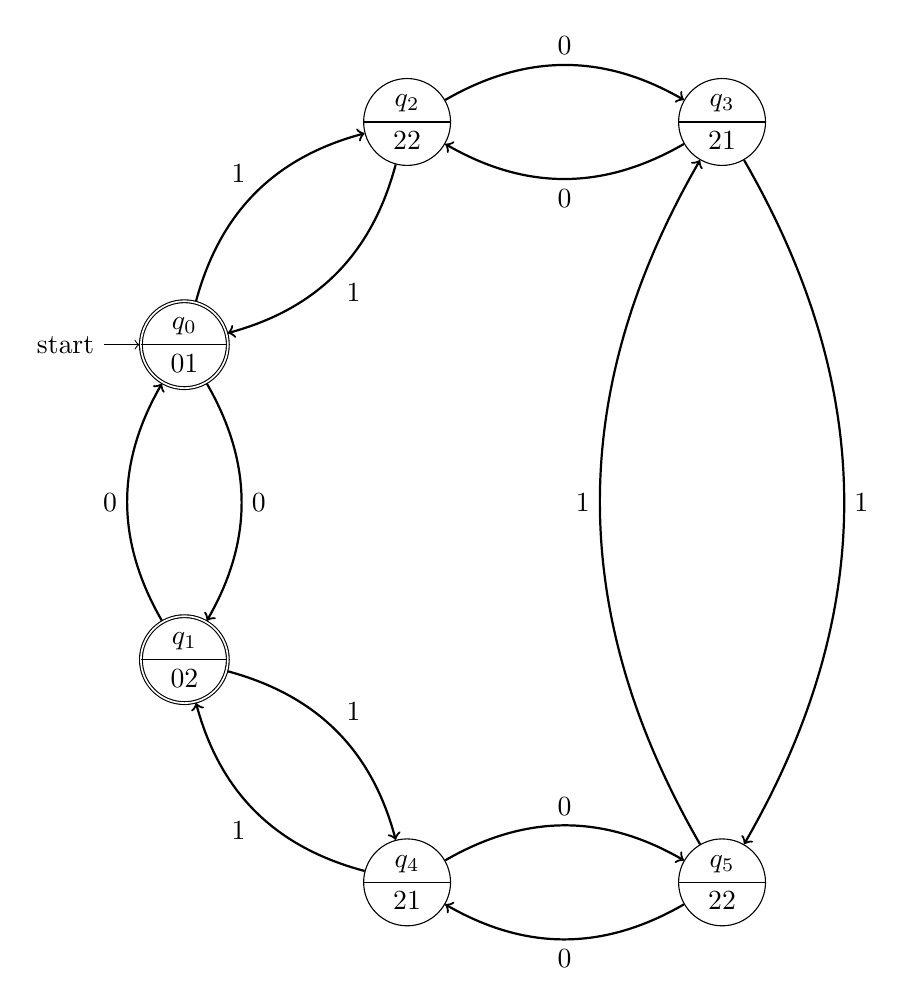
\begin{tikzpicture} [node distance = 4cm, on grid, auto]
       \node (q0) [state with output, initial, accepting]    {$q_0$ \nodepart{lower} $01$}; 
       \node (q1) [state with output,accepting]  [below = of q0] {$q_1$ \nodepart{lower} $02$}; 
       \node (q2) [state with output]  [above right= of q0] {$q_2$ \nodepart{lower} $22$};
       \node (q3) [state with output]  [right= of q2] {$q_3$ \nodepart{lower} $21$};
       \node (q4) [state with output]  [below right= of q1] {$q_4$ \nodepart{lower} $21$};
       \node (q5) [state with output]  [right = of q4] {$q_5$ \nodepart{lower} $22$};
        \path[->, thick] 
        (q0) edge[bend left]  node {0} (q1)
        (q0) edge[bend left]  node {1} (q2)
        (q1) edge[bend left]  node {1} (q4)
        (q1) edge[bend left]  node {0} (q0)
        (q2) edge[bend left]  node {1} (q0)
        (q2) edge[bend left]  node {0} (q3)
        (q3) edge[bend left]  node {1} (q5)
        (q3) edge[bend left]  node {0} (q2)
        (q4) edge[bend left]  node {1} (q1)
        (q4) edge[bend left]  node {0} (q5)
        (q5) edge[bend left]  node {0} (q4)
        (q5) edge[bend left]  node {1} (q3);
     \end{tikzpicture}
\caption{DFA for detecting, reading binary digits right-to-left, a number divisible by 3.}
\end{figure}

\end{document}